\begin{frame}
\frametitle{NLG Tasks (cont'd)}

\begin{columns}

	\begin{column}{0.4\textwidth}
		\centering
		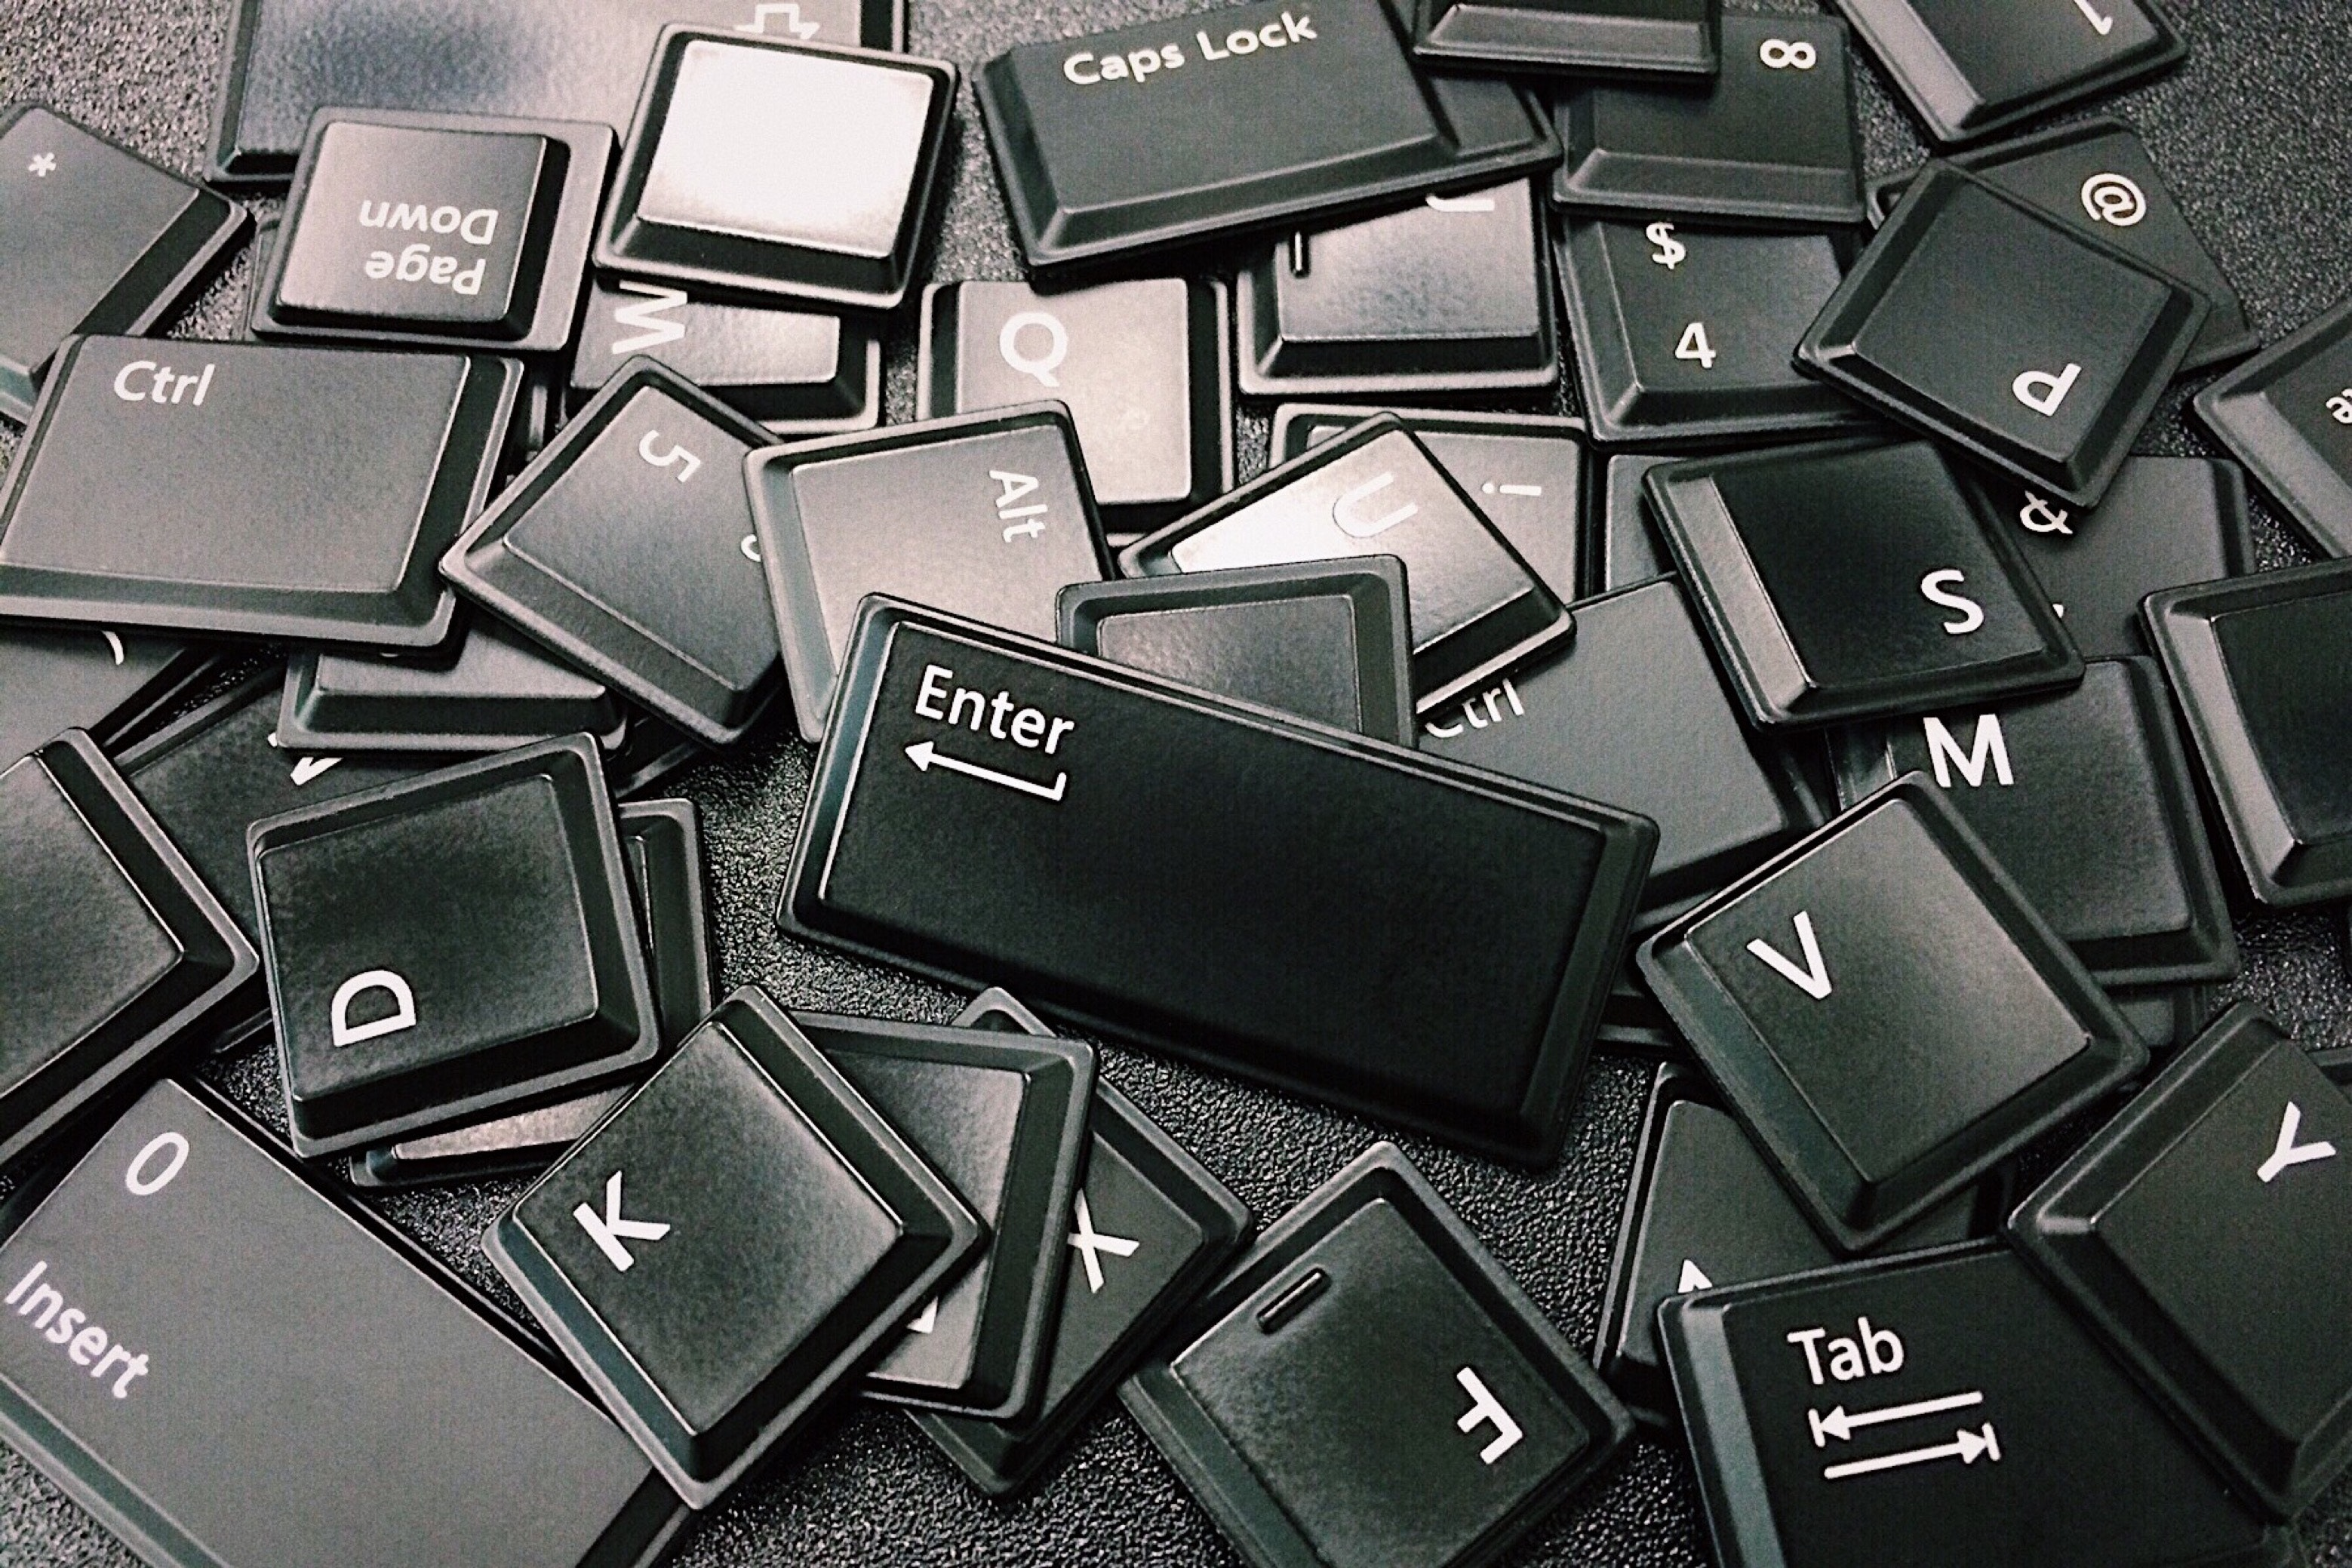
\includegraphics[angle=90,width=0.8\textwidth]{pexels-pixabay-373072}
	\end{column}
	
	\begin{column}{0.6\textwidth}
	
		\begin{itemize}
		
			\item \textbf{Lexicalization} \\
			      Choose specific words and phrases
			      to convey the concepts and relations
			      appearing in the messages
			      
			\item \textbf{Referring expression generation} \\
			      Select words or phrases to identify domain entities
			
			\item \textbf{Linguistic realisation} \\
			      Apply the rules of grammar to produce text
		
		\end{itemize}
		
		\vspace{12pt}
		
		A given task may be very complex in some systems,\\
		and very simple in others.
		
		\vspace{12pt}
		
		It depends on the requirements!
	
	\end{column}

\end{columns}

\end{frame}
